\documentclass[a4paper,12pt]{report}

\usepackage{cmap} % поиск в документе
\usepackage[T2A]{fontenc} % кодировка
\usepackage[utf8]{inputenc} % кодировка исходного текста
\usepackage[english, russian]{babel} % локализация и переносы

\usepackage{hyperref} % гиперссылки
\usepackage{ulem} % перечёркнутый текст
\usepackage{graphicx}  % Для вставки рисунков
\usepackage{indentfirst} % отступ после заголовка
\usepackage[labelsep=period]{caption} % : -> . в caption

\author{Колобов Кирилл, 201-321}
\date{}
\title{Аборты: геноцид или выбор?}

\begin{document}
\maketitle
\tableofcontents


\part{Введение}
Аборты -- частая причина разногласий между умудрённым опытом, годами старшим поколением 
с консервативными взгядами и идеологически прокачанными детьми.

Здесь разбираются основные положения споров, показывается аргументативная несостоятельность одной из сторон.


\part{За аборты}
\chapter{Позиция}
    Пока не родился -- не человек, аборт можно делать на любом сроке по любой причине.
\chapter{Доводы}
    \section{Зигота -- не человек}
        Зигота не является человеком, это всего лишь кусок мяса.
    \section{Человек начинается с рождения}
        Зародыш становится человеком после рождения, ребёнок получает свидетельство о рождении.
    \section{Зигота -- часть тела матери}
        Зигота не может существовать вне тела матери, без потпитки оттуда $\Rightarrow$ зигота -- часть тела матери.
    \section{У зиготы нет разума, нет сознания}
        Зигота не разумна, она не может реагировать ни на какие раздражители извне.
    \section{Зигота -- не личность}
        У зиготы не мозга, она ещё не сформировалась, она не личность.
    \section{У матери есть выбор}
        Женщина хочет убить паразита, чтобы не кормить его и не мучаться.
    \section{Ты хочешь плодить нищету?}
        Если ребёнок родится, то он будет жить в нищите, он будет нежеланным. Ты этого хочешь?
    \section{Мать не хотела заводить ребёнка}
        Мать не хотела заводить ребёнка, она против этого, она ещё не готова.
    \section{Мужчина не может рассуждать об этом}
        Мужчина не может решать за женщину, что и как ей делать.   
    \section{По закону можно}
        Какие могут быть вопросы, если законом разрешено?
    \section{А если это было изнасилование?}
        А если это было изнасилование, то тоже нельзя сделать аборт? Женщине рожать ребёнка от насильника?


\chapter{Выводы}
Здесь описаны какие-то выводы


\part{Против абортов}
\chapter{Позиция}
Здесь рассматриваются доводы с позиции гипотетической индукции: если можно убить плод, то можно убить 
уже родившегося человека в любом возрасте по тем же причинам, по которым делается аборт,
поскольку качественно человек не меняется с самого момента зачатия, см. пункт \ref{ishuman}.

Однако, сторонники аборотов старательно избегают последовательных рассуждений, 
допуская убийство плода, но выступая против убийства уже рождённых людей, что есть лицемерие,
перетекающее в геноцид.

Часть доказательств в кратком изложении представлены ниже. 

\chapter{Доводы}
    \section{Зигота -- человек}\label{ishuman}
        \begin{figure}[!h]
            \centering
            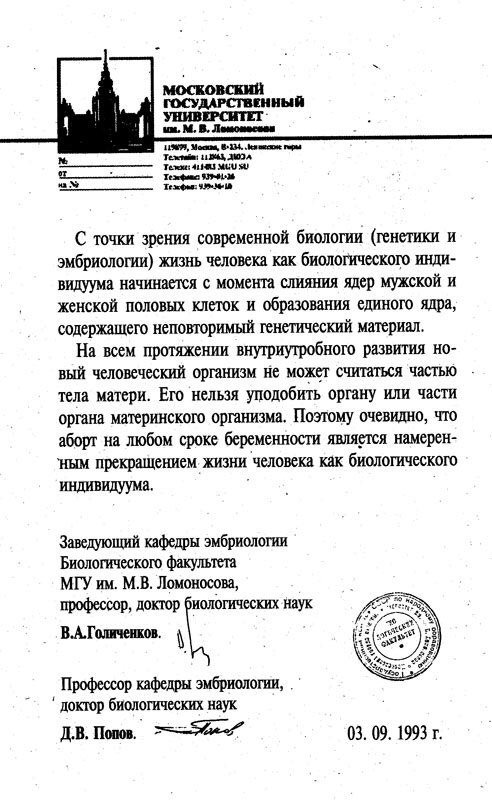
\includegraphics[width=0.45\textwidth]{evidence.jpg}
            \caption{Биологические данные}
        \end{figure}
     
        Человек -- представитель биологического вида \textit{Homo Sapiens Sapiens}, зигота принадлежит к этому виду $\Rightarrow$ зигота -- человек $\Rightarrow$ аборт -- убийство человека.
	\section{Человек начинается с зачатия}
        Зигота -- это первая стадия развития человеческого организма, см. пункт \ref{ishuman}. 
        Любое небиологическое деление -- арбитрарное, не имеет верифицируемых критериев. 

        Невалидность апеляций к законам рассмотрена ниже, пункт \ref{laws}.
	\section{Зигота -- новый организм}
        См. пункт \ref{ishuman}. Зигота -- первая стадия развития человека.

        А также, ребёнок не может жить без матери первые несколько лет после рождения. Однако оппоненты считают, что после рождения убивать нельзя.
        Выходит, этот довод используется непоследовательно, то есть противоречит их позиции.
    \section{Сторонники абортов -- нацисты}\label{nazi}
        В пресуппозициях к таким утверждениям, очевидно, есть следующее положение: 
        <<неразумных>> людей, людей без <<сознания>> можно убивать. 
	    Выходит, сторонники абортов за убийство всех людей с врождёнными или 
        пробритёнными отклонениями: слабоумие, старческая деменция, микроцефалия, 
        анэнцефалия\footnote{Отсутствие больших полушарий.}, вегетативная 
        кома\footnote{Состояние, из которого нельзя выйти, поскольку мозг 
        мёртв. Человек становится овощем.}. 
        Выходит, они не против убийства своей бабушки из-за \sout{жажды наследства} 
        её деменции на почве возраста. Это ли не нацизмом называется?
        
        Вообще говоря, из-за несформировавшегося мозга зигота не перестаёт относиться к 
        биологическому виду \textit{Homo Sapiens Sapiens}, то есть не перестаёт быть человеком.
    \section{А как проверить?}
        У этого параметра нет критериев верификации, аналогично <<сознанию>> из пункта \ref{nazi}.
	\section{Можно убить новорождённого?}
        Если у неё есть выбор, то может ли она убить новорождёного? 
        Если вы считаете, что может, то \sout{вы нацист} аборты, как и любое другое 
        убийство по сиюминутной прихоти, допустимы в рамках ваших ценностей, а 
        если нет -- аборты недопустимы.
    \section{А чем думала мать?}\label{thing-about-it}
        У неё был выбор, она могла отказаться от незащищённого секса. Однако не отказалась, 
        теперь пусть несёт ответственность за свои ошибки. Это не повод убивать кого-то.
	\section{А чем думала мать?}
        Аналогично пункту \ref{thing-about-it}.
    \section{А вы знаете, может}
        Может и последние несколько тысяч лет решает. В любом случае апелляции к полу невалидны.
    \section{В III Рейхе...}\label{laws}
        Апелляции к законам опять же невалидны, поскольку законы устанавливаются группой 
        людей исходя из их интересов.
	\section{Тогда можно}
        В таком случае аборт допустим, как и в случае угрозы жизни роженицы.


\chapter{Выводы}
Проблемы абортов, их распространённость и необходимость, у многих наслуху неспроста: 
современному среднечеловеку чуждо чувство отвественности, он не готов ни думать о 
своих действиях заранее, ни принимать последствия совершённых ошибок -- незащищённого 
секса, в данном случае.

Решение этой проблемы неоскорблённые умом видят в массовом геноциде определённой 
группы людей, самых незащищённых из нас --  нерождённых. 

При этом, к сожалению, процесс мышления (как и любовь до гроба, крепкая семья) из 
моды выходит, вследствие этого простая альтернатива гуляет перед лицом у \textit{homo consumer} 
незамеченной. 

Впрочем, предлагаемая альтернатива решит также проблему неизлечимых (а впрочем, 
излечимых тоже) венирических болезней: ВИЧ, его запущенная форма -- СПИД, 
сифилис, хламидиоз, трихомониаз et cetera.

И альтернатива эта (барабанная дробь!) -- защищённый секс.
\end{document}
